\documentclass[tikz, margin=.25mm]{standalone}
\usepackage[utf8x]{inputenc}
\usetikzlibrary{calc,arrows,fadings,decorations.pathreplacing,decorations.markings,patterns,shapes.geometric}

\begin{document}
    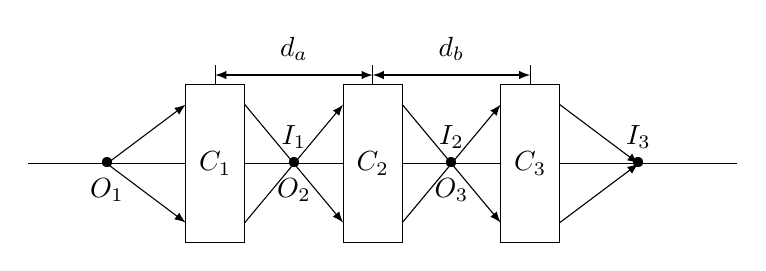
\begin{tikzpicture}[scale=1, outer sep=2pt,>=latex]
        \draw[] (0,0) -- +(9,0) ;
        \draw(1,0)node{•}node[below]{$O_1$};
        \draw(7.75,0)node{•}node[above]{$I_3$};
        \foreach \x in {1,2,3}{\draw[draw=black,fill=white] (2*\x,-1) rectangle ++(.75,2);}
        \node[] at (2.375,0) {$C_1$};
        \node[] at (4.375,0) {$C_2$};
        \node[] at (6.375,0) {$C_3$};
        \draw[<->] (2.375,1.125) -- ++(2,0)node[midway,above]{$d_a$};
        \draw[<->] (4.375,1.125) -- ++(2,0)node[midway,above]{$d_b$};
        \draw[-] (2.375,1) -- ++(0,.25);
        \draw[-] (4.375,1) -- ++(0,.25);
        \draw[-] (6.375,1) -- ++(0,.25);
        \draw[->] (1,0) -- ++(1,.75);
        \draw[->] (1,0) -- ++(1,-.75);
        \draw[->] (2.75,-0.75) -- ++(2-.75,1.5)node[midway]{•}node[midway,above]{$I_1$} node[midway,below]{$O_2$};
        \draw[->] (2.75,.75) -- ++(2-.75,-1.5);
        \draw[->] (4.75,-0.75) -- ++(2-.75,1.5)node[midway]{•}node[midway,above]{$I_2$} node[midway,below]{$O_3$};
        \draw[->] (4.75,.75) -- ++(2-.75,-1.5);
        \draw[->] (6.75,.75) -- ++(1,-.75);
        \draw[->] (6.75,-.75) -- ++(1,.75);
    \end{tikzpicture}  
\end{document}